% ==============================================================================



\documentclass[../../../Master/AppliedStochastics.tex]{subfiles}



% ==============================================================================


\author{Chandler}
\date{03 October 2018}


% ==============================================================================
%
\begin{document}
%
% ==============================================================================


\makelecture


\section{An Application}

We operate a cufflink machine:


\begin{center}
	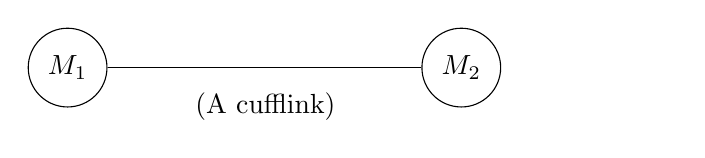
\begin{tikzpicture}
	\node[circle,draw, minimum size=1cm] (M1) at (0,0) {$M_1$};
	\node[circle,draw, minimum size=1cm] (M2) at (5,0) {$M_2$};
	\draw (M1) -- (M2);
	\node[text width=6cm, anchor=west, right] at (1.5,-.5) {(A cufflink)};
	\end{tikzpicture}
\end{center}


The weights of the two ends,
    $M_1$ and $M_2$ are $i.i.d\ N(5,10)$.
We want to only keep cufflinks that are balanced. 
That means $\abs{M_{1} - M_{2}}$ is small.


\textbf{A}.
It's easy to weigh both ends, $M_{1}+M_{2}$. 
Does this help identify the bad cufflinks?


\textcolor{Red}{
    No.
    $M_{1}+M_{2}$ and $M_{1}-M_{2}$ are independent. 
	This is because: 
	$$\begin{aligned}
	   \cov [M_{1}+M_{2}, M_{1}-M_{2}] = \var [M_{1}]-\var [M_{2}] = 0\,.
	\end{aligned}$$}

\textbf{B}.
What is the distribution of $M_{1}$ among cufflinks with
    $M_{1}+M_{2}\approx 12$? 

\textcolor{Red}{
    Let $A=M_{1}+M_{2}$ and $B=M_{1}-M_{2}$, then $M_{1}=\frac{A+B}{2}$.
    From Part A we know $A$ and $B$ are independent.
	$$\begin{aligned}
	   (M_{1}\vert A=12) \stackrel{d}{=} \dfrac{12 + B}{2} \sim N(6,2)
	\end{aligned}$$
	This result follows from the fact that: 
	$$\begin{aligned}
	   B \sim N(0,2)
	\end{aligned}$$ 
	   since $B=M_{1}-M_{2}$.}


\section{Conditional Distributions}


\begin{lemma}[Conditional Distributions]
Let $\underset{n\times n}{X}$ and $\underset{m\times m}{Y}$ be
    jointly Gaussian with mean zero and covariance: 
$$\begin{aligned}
\begin{bmatrix}
  	\underset{n\times n}{\Sigma_{XX}} & \underset{m\times n}{\Sigma_{XY}} \\ 
   	\underset{n\times m}{\Sigma_{XY}\trans} & \underset{m\times m}{\Sigma_{YY}}
\end{bmatrix}
\end{aligned}$$

\begin{note} 
\end{note} 

Then, 
$$\begin{aligned}
\E[X\vert Y] = \Sigma_{XY}\Sigma_{YY}^{-1} Y
\end{aligned}$$
and 
$$\begin{aligned}
    (X\vert Y=y) \sim N(\Sigma_{XY}\Sigma_{YY}\inv, 
    \Sigma_{XX} - \Sigma_{XY} \Sigma_{YY}\inv \Sigma_{XY}\trans)
\end{aligned}$$
Note that if $\Sigma_{YY}$ is not invertible,
    we may use the Moore-Penrose inverse.
That is, the above equations then remain true if the inverse used
        is the Moore-Penrose generalized inverse.
Further,
    note that $\Sigma_{XX} - \Sigma_{XY} \Sigma_{YY}\inv \Sigma_{XY}\trans$
    is the Schur complement of our covariance matrix.
\end{lemma}



\begin{proof}
Let $A = \Sigma_{XY} \Sigma_{YY}\inv Y$ and $X = A + B$. 
Claim: $B$ is independent of $Y$.\todo{Is this line correct?}
$$\begin{aligned}
\cov[X - \Sigma_{XX} \Sigma_{YY}\inv Y, Y]
    = \cov[X, Y]
    = \cov[X, Y] - \Sigma_{XY} \Sigma_{YY}\inv \cov[Y, Y]  
 = 0\,.
\end{aligned}$$
Now we can say: 
$$\begin{aligned}
(X \vert Y = y) \stackrel{d}{=} \Sigma_{XY}\Sigma_{YY}\inv y + B 
\end{aligned}$$
To confirm that this is the same distribution as before
    we need to calculate: 
$$\begin{aligned}
    \cov[B, B] = \cov[X - \Sigma_{XY} \Sigma_{YY}\inv Y,
        X - \Sigma_{XY} \Sigma_{YY}\inv Y]\\
        = \cov[X, X] - \cov[X, Y] \Sigma_{YY}\inv \Sigma_{XY}\trans
            - \Sigma_{XY} \Sigma_{YY}\inv \cov[Y, X]
            + \Sigma_{XY} \Sigma_{YY}\inv \cov[Y, Y]
                \Sigma_{YY}\inv \Sigma_{XY}\trans \\
        = \Sigma_{XX} - \Sigma_{XY} \Sigma_{YY}\inv \Sigma_{XY}\trans
\end{aligned}$$
Thus,
    $(X \vert Y = y) \sim N(\Sigma_{XY}\Sigma_{YY}\inv,
        \Sigma_{XX} - \Sigma_{XY} \Sigma_{YY}\inv \Sigma_{XY}\trans)$.
\end{proof}


\section{Gaussian Process Regression}


Suppose we have a random curve that is drawn from a Gaussian process. 
We observe the value of this process at a few noisy points. 
\begin{center}
	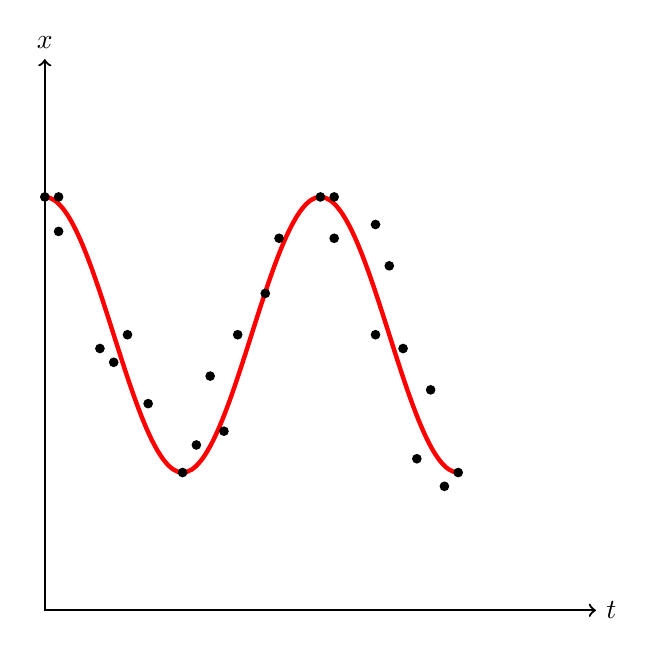
\begin{tikzpicture}[scale=1.75]
	\draw [<->,thick] (0,2) node (yaxis) [above] {$x$}|- (4,-2) node (xaxis) 
	[right] {$t$};
	\draw[x=0.5cm,y=1cm, ultra thick, red](0,1) cos (1,0) sin (2,-1) cos (3,0) 
	sin (4,1) cos (5,0) sin (6,-1);
	
	
	\foreach \point in 
	{(0,1),(.1,1),(.1,.75),(.6,0),(.4,-.1),(.5,-.2),(.75,-.5),(1,-1),(1.1,-.8),(1.2,-.3),(1.3,-.7),(1.4,0),(1.6,.3),(1.7,.7),
	 (2,1), (2.1,1), (2.1,.7), (2.4,0), (2.4,.8), 
	(2.5,.5),(2.6,-.1),(2.7,-.9),(2.8,-.4),(2.9,-1.1),(3,-1)}{% points
		\fill \point circle (1pt);
	}
	\end{tikzpicture}
\end{center}
Using this information we can find out more about this curve, 
including confidence intervals about points. 

But, first we'll look more at the Brownian Bridge. 
Recall (for $0\leq t < 1$), 

$$\begin{aligned}
U_{t} = (B_{t}\vert B_{1}=0) \stackrel{d}{=} B_{t} - tB_{1} 
\end{aligned}$$

Check this, 
$$\begin{aligned}
\cov[B_{1}, B_{t}-tB_{1}]= t - t\cdot 1 = 0 
\end{aligned}$$

Recall, 
$$\begin{aligned}
U_{t}=B_{t}-Z_{0,0}\int_{0}^{t}h_{0}(s)ds=Z(\mathbf{1}_{[0,t)})) - tZ_{0,0} = 
\sum_{n\geq1}\sum_{k=1}^{2^n}Z_{n,k}\int_{0}^{t} h_{n,k}(s)ds
\end{aligned}$$

What is the distribution of $U_{t}-U_{s}$ ? (for $s<t$)
$$\begin{aligned}
U_{t}-U_{s} = \sum_{n\geq1}\sum_{k=1}^{2^n} Z_{n,k}\int_{s}^{t} h_{n,k}(s)ds = 
Z(\mathbf{1}_{[s,t)})-(t-s)Z_{0,0}
\end{aligned}$$
So, 
$$\begin{aligned}
\var[U_{t}-U_{s}] = \var[Z(\mathbf{1}_{[s,t)})]- 
2(t-s)\cdot\cov[Z(\mathbf{1}_{[s,t)}),Z(\mathbf{1}_{[0,1)})] + (t-s)^2 \cdot 
\var[Z(\mathbf{1}_{[0,1)})]
\end{aligned}$$
Note that, 
$$\begin{aligned}
\var[Z(\mathbf{1}_{[s,t)})] = \int_{0}^{1} \mathbf{1}_{[s,t)}(u) \cdot 
\mathbf{1}_{[s,t)}(u) du = t-s 
\end{aligned}$$
So, we'll have 
$$\begin{aligned}
\var[U_{t}-U_{s}] = (t-s) - 2(t-s)^2 + (t-s)^2 = (t-s)[1-(t-s)]
\end{aligned}$$
Thus, 
$$\begin{aligned}
U_{t}-U_{s} \sim N\Big(0, (t-s)[1-(t-s)]\Big)
\end{aligned}$$


% ==============================================================================
%
\end{document}
%
% ==============================================================================
